\documentclass[]{article}
\usepackage[brazilian]{babel}
\usepackage[utf8]{inputenc}
\usepackage[T1]{fontenc}
\usepackage{fancyhdr}
\usepackage{extramarks}
\usepackage{amsmath}
\usepackage{amsthm}
\usepackage{amsfonts}
\usepackage{tikz}
% \usepackage[plain]{algorithm}
\usepackage{algpseudocode}
\usepackage{listings}
\usepackage{xcolor}
\usepackage{listings}
\usepackage{amssymb}

\usepackage{caption}

\usepackage{tikz}
\newcommand*\circled[1]{\tikz[baseline=(char.base)]{
            \node[shape=circle,draw,inner sep=2pt] (char) {#1};}}

\usepackage{enumitem}

\usepackage[ruled,portuguese,onelanguage,longend]{algorithm2e} %for psuedo code}% http://ctan.org/pkg/algorithm2e





\definecolor{mGreen}{rgb}{0,0.6,0}
\definecolor{mGray}{rgb}{0.5,0.5,0.5}
\definecolor{mPurple}{rgb}{0.58,0,0.82}
\definecolor{backgroundColour}{rgb}{0.95,0.95,0.92}

\lstdefinestyle{CStyle}{
    belowcaptionskip=1\baselineskip,
    breaklines=true,
    frame=L,
    xleftmargin=\parindent,
    language=C,
    showstringspaces=false,
    basicstyle=\footnotesize\ttfamily,
    keywordstyle=\bfseries\color{green!40!black},
    commentstyle=\itshape\color{purple!40!black},
    identifierstyle=\color{blue},
    stringstyle=\color{orange},
}

\usetikzlibrary{automata,positioning}

%
% Basic Document Settings
%

\topmargin=-0.45in
\evensidemargin=0in
\oddsidemargin=0in
\textwidth=6.5in
\textheight=9.0in
\headsep=0.25in

\linespread{1.1}

\pagestyle{fancy}
\lhead{AVC, JPP, PC}
\chead{\hmwkClass\ (\hmwkClassInstructor\ \hmwkClassTime): \hmwkTitle}
\rhead{\firstxmark}
\lfoot{\lastxmark}
\cfoot{\thepage}

\renewcommand\headrulewidth{0.4pt}
\renewcommand\footrulewidth{0.4pt}

\setlength\parindent{0pt}

%
% Create Questão Sections
%

\newcommand{\enterProblemHeader}[1]{
    \nobreak\extramarks{}{Questão \arabic{#1} continua na próxima página\ldots}\nobreak{}
    \nobreak\extramarks{Questão \arabic{#1} (cont.)}{Questão \arabic{#1} continua na próxima página\ldots}\nobreak{}
}

\newcommand{\exitProblemHeader}[1]{
    \nobreak\extramarks{Questão \arabic{#1} (cont.)}{Questão \arabic{#1} continua na próxima página\ldots}\nobreak{}
    \stepcounter{#1}
    \nobreak\extramarks{Questão \arabic{#1}}{}\nobreak{}
}

\setcounter{secnumdepth}{0}
\newcounter{partCounter}
\newcounter{homeworkProblemCounter}
\setcounter{homeworkProblemCounter}{1}
\nobreak\extramarks{Questão \arabic{homeworkProblemCounter}}{}\nobreak{}

%
% Homework Questão Environment
%
% This environment takes an optional argument. When given, it will adjust the
% problem counter. This is useful for when the problems given for your
% assignment aren't sequential. See the last 3 problems of this template for an
% example.
%
\newenvironment{homeworkProblem}[1][-1]{
    \ifnum#1>0
        \setcounter{homeworkProblemCounter}{#1}
    \fi
    \section{Questão \arabic{homeworkProblemCounter}}
    \setcounter{partCounter}{1}
    \enterProblemHeader{homeworkProblemCounter}
}{
    \exitProblemHeader{homeworkProblemCounter}
}

%
% Homework Details
%   - Title
%   - Due date
%   - Class
%   - Section/Time
%   - Instructor
%   - Author
%

\newcommand{\hmwkTitle}{Lista 2}
\newcommand{\hmwkDueDate}{xx de novembro de 2019}
\newcommand{\hmwkClass}{Programação Modular}
\newcommand{\hmwkClassTime}{}
\newcommand{\hmwkClassInstructor}{Professor Flavio Bevilacqua}

% \setlength{\textfloatsep}{1in}
\newcommand{\hmwkAuthorName}{

\begin{tabular}{c}\textbf{Antônio Vasconcellos Chaves} \\ Engenharia da Computaçāo \\ Pontifícia Universidade Católica \\ do Rio de Janeiro \\ Rio de Janeiro, RJ 22451-900 \\ antoniovasconcelloschaves@gmail.com \end{tabular}\and

\begin{tabular}{c}\textbf{João Pedro Paiva} \\ Ciência da Computaçāo \\ Pontifícia Universidade Católica \\ do Rio de Janeiro \\ Rio de Janeiro, RJ 22451-900 \\ joaopedrordepaiva@gmail.com \end{tabular}\and

\\[\baselineskip]\begin{tabular}{c}\textbf{Pedro Moreira Costa} \\ Engenharia da Computaçāo \\ Pontifícia Universidade Católica \\ do Rio de Janeiro \\ Rio de Janeiro, RJ 22451-900 \\ pedromoreiramcosta@gmail.com \end{tabular}

}

%
% Title Page
%

\title{
    \vspace{2in}
    \textmd{\textbf{\hmwkClass:\ \hmwkTitle}}\\
    \normalsize\vspace{0.1in}\small{Entrega\ no dia\ \hmwkDueDate\ às 17h}\\
    \vspace{0.1in}\large{\textit{\hmwkClassInstructor\ \hmwkClassTime}}
    \vspace{1.25in}
}

\author{\hmwkAuthorName}
\date{}

\renewcommand{\part}[1]{\textbf{\large Parte \Alph{partCounter}}\stepcounter{partCounter}\\}

%
% Various Helper Commands
%

% Useful for algorithms
\newcommand{\alg}[1]{\textsc{\bfseries \footnotesize #1}}

% For derivatives
\newcommand{\deriv}[1]{\frac{\mathrm{d}}{\mathrm{d}x} (#1)}

% For partial derivatives
\newcommand{\pderiv}[2]{\frac{\partial}{\partial #1} (#2)}

% Integral dx
\newcommand{\dx}{\mathrm{d}x}

% Alias for the Solution section header
\newcommand{\solution}{\textbf{\large Solução}}

% Probability commands: Expectation, Variance, Covariance, Bias
\newcommand{\E}{\mathrm{E}}
\newcommand{\Var}{\mathrm{Var}}
\newcommand{\Cov}{\mathrm{Cov}}
\newcommand{\Bias}{\mathrm{Bias}}

\begin{document}

\SetEndCharOfAlgoLine{}

\maketitle

\pagebreak

\begin{homeworkProblem}

    Apresente a estrutura de decomposição sucessiva do algoritmo de quicksort apontando um componente concreto, um componente abstrato e um conjunto solução.

    \vspace{\baselineskip}
    \textbf{Solução}

    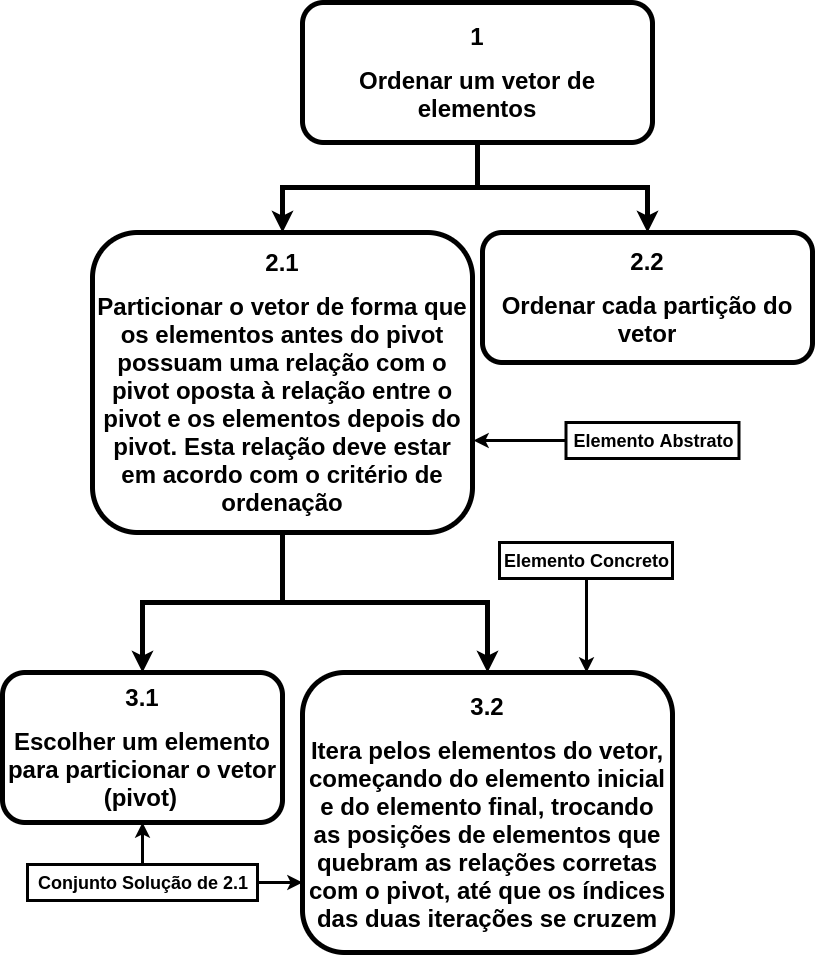
\includegraphics[width=\textwidth]{Q1.png}

\end{homeworkProblem}

\vspace{\baselineskip}

\begin{homeworkProblem}

    Faça a argumentação de corretude completa de uma pesquisa binária em um vetor.

    \vspace{\baselineskip}
    \textbf{Solução}

    \begin{algorithm}[h]

        \caption{Busca Binária em Vetor}

        \SetAlgoLined
        % \KwData{this text}
        % \KwResult{how to write algorithm with \LaTeX2e }
        AE $\longrightarrow$

        \Indp\Inicio
        {

            COMEÇO $\longleftarrow$ 1

            FINAL $\longleftarrow$ LIMITE-LÓGICO

            \Enqto{COMEÇO $\leq$ FINAL}
            {

                ATUAL $\longleftarrow$ (COMEÇO + FINAL) / 2

                \lSe{VETOR[ATUAL] == PARÂMETRO-BUSCADO}{\Retorna ATUAL}

                \lSe{VETOR[ATUAL] < PARÂMETRO-BUSCADO}{COMEÇO $\longleftarrow$ ATUAL + 1}

                \lSenao{FINAL $\longleftarrow$ ATUAL - 1}

            }

            \Retorna{-1}

        }

        \Indm AS $\longrightarrow$

    \end{algorithm}

    \textbf{Argumentação de Sequência 1}

    AE: Existe um número a ser buscado em um vetor ordenado.

    AS: PARÂMETRO-BUSCADO está na posição retornada, ou não está no vetor e o valor retornado é -1.

    AI 1: COMEÇO aponta para o primeiro elemento do vetor.

    AI 2: FINAL aponta para o LIMITE-LÓGICO do vetor.

    AI 3: PARÂMETRO-BUSCADO não está no vetor.

    \textbf{Argumentação de Repetição 1}

    AE: AI 2.

    AS: PARÂMETRO-BUSCADO está na posição retornada, ou não está no vetor.

    AINV:

    \begin{itemize}

        \item Existem dois conjuntos: pode conter PARÂMETRO-BUSCADO e não contém PARÂMETRO-BUSCADO.
        \item COMEÇO e FINAL apontam para os limites inferior e superior, respectivamente, do conjunto pode conter PARÂMETRO-BUSCADO.

    \end{itemize}

    \begin{enumerate}[label=\protect\circled{\arabic*}]
        \item AE $\Longrightarrow$ AINV

              \begin{itemize}
                  \item Pela AE, FINAL aponta para o LIMITE-LÓGICO do vetor. Todos os elementos estão no conjunto pode conter PARÂMETRO-BUSCADO e o conjunto não contém PARÂMETRO-BUSCADO está vazio. Logo, vale a AINV.
              \end{itemize}

        \item AE \&\& (Condição == False) $\Longrightarrow$ AS

              \begin{itemize}
                  \item Pela AE, FINAL aponta para o LIMITE-LÓGICO do vetor. Para que (Condição == False), FINAL < COMEÇO. Já que COMEÇO == 1, FINAL == 0. Logo, LIMITE-LÓGICO == 0, ou seja, o vetor está vazio. Neste caso, vale a AS, já que o PARÂMETRO-BUSCADO não está no vetor.
              \end{itemize}

        \item AE \&\& (Condição == True) \circled{+} B $\Longrightarrow$ AINV

              \begin{itemize}
                  \item Pela AE, FINAL aponta para o LIMITE-LÓGICO do vetor. Para que  (Condição == True), o vetor possui ao menos um elemento. Metade dos elementos do conjunto pode conter PARÂMETRO-BUSCADO passarão para o conjunto não contém PARÂMETRO-BUSCADO, e COMEÇO e FINAL serão reposicionados, apontando para os limites do novo conjunto pode conter PARÂMETRO-BUSCADO. Com isso, os dois conjuntos existem e COMEÇO e FINAL apontam para os limites do conjunto pode conter PARÂMETRO-BUSCADO. Logo, vale a AINV.s
              \end{itemize}

        \item AINV \&\& (Condição == True) \circled{+} B $\Longrightarrow$ AINV

              \begin{itemize}
                  \item Para que a AINV continue valendo, B deve garantir que metade dos elementos do conjunto pode conter PARÂMETRO-BUSCADO passem para o conjunto não contém PARÂMETRO-BUSCADO, e COMEÇO e FINAL sejam reposicionados, apontando para os limites do novo conjunto pode conter PARÂMETRO-BUSCADO.
              \end{itemize}

        \item AINV \&\& (Condição == False) \circled{+} B $\Longrightarrow$ AS

              \begin{itemize}
                  \item Se (Condição == False), o limite inferior do conjunto pode conter PARÂMETRO-BUSCADO superou o limite superior, ou seja, todos os elementos passaram para o conjunto não contém PARÂMETRO-BUSCADO e o conjunto pode conter PARÂMETRO-BUSCADO está vazio. Como o PARÂMETRO-BUSCADO não está no vetor, vale a AS.
              \end{itemize}

        \item Término

              \begin{itemize}
                  \item Como a cada ciclo, metade dos elementos do conjunto pode conter PARÂMETRO-BUSCADO são retirados, e este conjunto possui um número finito de elementos, a repetição terminará em um número finito de passos.
              \end{itemize}

    \end{enumerate}

    \textbf{Argumentação de Sequência 2}

    AE (seq2) = AS (seq2) = AINV.

    AI 4: ATUAL aponta para o meio do conjunto pode conter PARÂMETRO-BUSCADO.

    \textbf{Argumentação de Seleção 1}

    AE: AI 4.

    AS: AINV ou AS geral.

    \begin{enumerate}[label=\protect\circled{\arabic*}]
        \item AE \&\& (Condição == True) \circled{+} B1 $\Longrightarrow$ AS

              Pela AE, ATUAL aponta para o meio do conjunto pode conter PARÂMETRO-BUSCADO. Como (Condição == True), ATUAL aponta para o PARÂMETRO-BUSCADO. Neste caso, executa B1 que retorna a posição de PARÂMETRO-BUSCADO, valendo a AS.

        \item AE \&\& (Condição == False) \circled{+} B2 $\Longrightarrow$ AS

              Pela AE, ATUAL aponta para o meio do conjunto pode conter PARÂMETRO-BUSCADO. Como (Condição == False), ATUAL não aponta para o PARÂMETRO-BUSCADO. Neste caso, executa B2 que passa metade dos elementos do conjunto pode conter PARÂMETRO-BUSCADO para o conjunto não contém PARÂMETRO-BUSCADO. Vale a AS pois COMEÇO e FINAL apontam para os limites inferior e superior, respectivamente, do conjunto pode conter PARÂMETRO-BUSCADO.

    \end{enumerate}

    \textbf{Argumentação de Seleção 2}

    AE (sel2) = AE (sel1) e ATUAL não aponta para o PARÂMETRO-BUSCADO.

    AS: AINV e metade inferior ou superior dos elementos do conjunto pode conter PARÂMETRO-BUSCADO foi passada para o conjunto não contém PARÂMETRO-BUSCADO.

    \begin{enumerate}[label=\protect\circled{\arabic*}]
        \item AE \&\& (Condição == True) \circled{+} B1 $\Longrightarrow$ AS

              Pela AE, ATUAL aponta para o meio do conjunto pode conter PARÂMETRO-BUSCADO mas não aponta para o PARÂMETRO-BUSCADO. Como (Condição == True), o elemento apontado por ATUAL é menor do que PARÂMETRO-BUSCADO. Neste caso, executa B1 que redefine COMEÇO, passando a metade inferior dos elementos do conjunto pode conter PARÂMETRO-BUSCADO para o conjunto não contém PARÂMETRO-BUSCADO e valendo a AS.

        \item AE \&\& (Condição == False) \circled{+} B2 $\Longrightarrow$ AS

              Pela AE, ATUAL aponta para o meio do conjunto pode conter PARÂMETRO-BUSCADO mas não aponta para o PARÂMETRO-BUSCADO. Como (Condição == False), o elemento apontado por ATUAL é maior ou igual que PARÂMETRO-BUSCADO. Neste caso, executa B2 que redefine FINAL, passando a metade superior dos elementos do conjunto pode conter PARÂMETRO-BUSCADO para o conjunto não contém PARÂMETRO-BUSCADO e valendo a AS.

    \end{enumerate}


\end{homeworkProblem}

\vspace{\baselineskip}

\begin{homeworkProblem}

    Escolha uma função do trabalho e distribua os controladores de cobertura pelo padrão cobertura de arestas.

    \vspace{\baselineskip}
    \textbf{Solução}

    \lstinputlisting[style=CStyle]{Q3.C}

\end{homeworkProblem}

\vspace{\baselineskip}

\begin{homeworkProblem}

    Transforme uma estrutura de matriz tridimensional criada com listas em autoverificável.

    \vspace{\baselineskip}
    \textbf{Solução}

\end{homeworkProblem}

\vspace{\baselineskip}

\begin{homeworkProblem}

    Elabore um verficador para a estrutura da questão quatro com três verificações de campos redundantes.

    \vspace{\baselineskip}
    \textbf{Solução}

\end{homeworkProblem}

\vspace{\baselineskip}

\begin{homeworkProblem}

    Apresente um deturpador utlizado para testar o verficador da questão cinco.

    \vspace{\baselineskip}
    \textbf{Solução}

\end{homeworkProblem}

\vspace{\baselineskip}

\begin{homeworkProblem}

    Apresente uma situação em que os casos de teste pelo padrão cobertura de comandos, decisões e arestas são exatamente iguais.

    \vspace{\baselineskip}
    \textbf{Solução}

    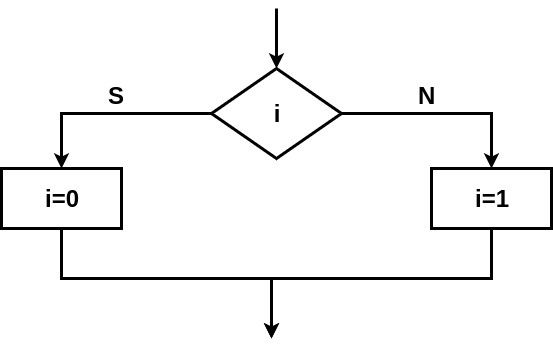
\includegraphics[width=\textwidth]{Q7.png}

\end{homeworkProblem}

\vspace{\baselineskip}

\begin{homeworkProblem}

    Qual é o arrasto de uma repetição existente em uma pesquisa binária recursiva?

    \vspace{\baselineskip}
    \textbf{Solução}

    2.

\end{homeworkProblem}

\vspace{\baselineskip}

\begin{homeworkProblem}

    Um controle de qualidade garante a corretude de um código quando seu teste é completo e não apresenta erros. Certo/Errado/Justifique.

    \vspace{\baselineskip}
    \textbf{Solução}

    Errado. O teste não apresentar erros significa que a implementação possui alta qualidade observada, mas não garante que a qualidade atestada seja igualmente alta caso a análise sobre o teste seja incorreta. Mesmo que o teste seja completo e a análise sobre o teste correta, não significa que o critério de seleção de casos de teste seja válido, o teste pode não acusar falhas quando há, ou confiável, o teste pode não paresentar erros por uma escolha específica ou ação feito em um dos casos de teste.

\end{homeworkProblem}

\vspace{\baselineskip}

\begin{homeworkProblem}

    Apresente todos os casos de teste do deturpador do trabalho 4 pelo padrão cobertura de arestas.

    \vspace{\baselineskip}
    \textbf{Solução}

    \bigskip

    \begin{tabular}{ | c | c c c c c c c c c c c c c c | }
        \hline
        Deturpação/Caso & 1  & 2  & 3  & 4  & 5  & 6  & 7  & 8  & 9  & 10 & 11 & 12 & 13 & 14 \\
        ==1             & S  & N  & N  & N  & N  & N  & N  & N  & N  & N  & N  & N  & N  & N  \\
        ==2             & NT & S  & N  & N  & N  & N  & N  & N  & N  & N  & N  & N  & N  & N  \\
        ==3             & NT & NT & S  & N  & N  & N  & N  & N  & N  & N  & N  & N  & N  & N  \\
        ==4             & NT & NT & NT & S  & N  & N  & N  & N  & N  & N  & N  & N  & N  & N  \\
        ==5             & NT & NT & NT & NT & S  & N  & N  & N  & N  & N  & N  & N  & N  & N  \\
        ==6             & NT & NT & NT & NT & NT & S  & N  & N  & N  & N  & N  & N  & N  & N  \\
        ==7             & NT & NT & NT & NT & NT & NT & S  & N  & N  & N  & N  & N  & N  & N  \\
        ==8             & NT & NT & NT & NT & NT & NT & NT & S  & N  & N  & N  & N  & N  & N  \\
        ==9             & NT & NT & NT & NT & NT & NT & NT & NT & S  & N  & N  & N  & N  & N  \\
        ==10            & NT & NT & NT & NT & NT & NT & NT & NT & NT & S  & N  & N  & N  & N  \\
        ==11            & NT & NT & NT & NT & NT & NT & NT & NT & NT & NT & S  & N  & N  & N  \\
        ==12            & NT & NT & NT & NT & NT & NT & NT & NT & NT & NT & NT & S  & N  & N  \\
        ==13            & NT & NT & NT & NT & NT & NT & NT & NT & NT & NT & NT & NT & S  & N  \\
        ==14            & NT & NT & NT & NT & NT & NT & NT & NT & NT & NT & NT & NT & NT & S  \\
        \hline
    \end{tabular}

    \bigskip

    S: sim

    N: não

    NT: não testa

\end{homeworkProblem}

\vspace{\baselineskip}

\begin{homeworkProblem}

    Utilizando o método de partição em classes de equivalência, gere o script para uma exclusão de nó corrente de uma árvore binária.

    \vspace{\baselineskip}
    \textbf{Solução}

    Passo 1: Árvore vazia, árvore com um único nível, árvore com três níveis (possui nível intermendiário).

    Resultados esperados: excluiu, não excluiu.

    \bigskip

    Passo 2:

    \bigskip

    \begin{tabular}{ c c c c c }

        Caso & Estrutura & Elemento a excluir & Excluiu & Não Excluiu \\
        \hline
        \hline
        S    & Vazia     & Primeiro           & N       & S           \\
        2    & A         & Raiz               & S       & N           \\
        3    & (A,(B,C)) & Raiz               & S       & N           \\
        4    & (A,(B,C)) & Filho à direita    & S       & N           \\
        5    & (A,(B,C)) & Filho à esquerda   & S       & 0
    \end{tabular}

    \bigskip

    Passo 3:

    \bigskip

    ==caso1

    =criaarvore	0

    =exclui		0

    \bigskip

    ==caso2

    =insere		A

    =exclui		0

    \bigskip

    ==caso3

    =insere		    A

    =insere		    B

    =insere		    C

    =irpai	        0

    =exclui		    0

    =liberaarvore	0

    \bigskip

    ==caso4

    =insere		    A

    =insere		    B

    =insere		    C

    =exclui		    0

    =liberalista	0

    \bigskip

    ==caso5

    =insere		    A

    =insere		    B

    =insere		    C

    =irpai		    0

    =iresq          0

    =exclui		    0

    =liberalista	0

\end{homeworkProblem}

\vspace{\baselineskip}

\begin{homeworkProblem}

    Apresente uma situação em que as qualidades efetiva e observada são diferentes.

    \vspace{\baselineskip}
    \textbf{Solução}

    Quando a implementação de um artefato é incorreta e o teste é incompleto, não abordando o aspecto incorreto da implementação, mas a análise dos resultados do teste é correta, a qualidade observada será alta, a qualidade atestada será baixa e a qualidade efetiva será baixa.

\end{homeworkProblem}

\vspace{\baselineskip}

\begin{homeworkProblem}

    Existe relação entre a abordagem de teste orientado à destruição e a qualidade atestada não se aproximar da qualidade requerida. Certo/Errado/Justifique.

    \vspace{\baselineskip}
    \textbf{Solução}

    A qualidade requerida aumenta quando nos aproximamos daquilo que o cliente quer. A qualidade atestada se refere ao que é descrito por um controle de qualidade. Ao utlizarmos a abordagem de teste orientado à destruição, examinamos somente se a implementação de algum artefato está correta, mas não se aquela é a implementação que o cliente deseja. Utlizando esta abordagem, garantimos que a implementação possua boa qualidade, mas não garantimos qualidade satisfatória.

\end{homeworkProblem}

\vspace{\baselineskip}

\begin{homeworkProblem}

    Explique porque é necessário utilizar campos redundantes ao instrumentar uma estrutura autoverificável.

    \vspace{\baselineskip}
    \textbf{Solução}

    Os dados redundantes ajudam na confiabilidade daquilo que foi implementado. Por exemplo, se colocarmos um campo que descreve o tipo da estrutura na cabeça da estrutura e nos nós, então podemos verificar se o nó pertence à estrutura pela combinação, ou não, do tipo apontado pelo nó e pela cabeça. A implementação de múltiplos campos com este mesmo objetivo, como um campo que descreve o tamanho do nó colocado na cabeça da estrutura e nos nós, enfatizará ainda mais a corretude da implementação.

\end{homeworkProblem}

\vspace{\baselineskip}


\end{document}
